\chapter{ゲージ場、相互作用のスケール、荷電弱カレント}

量子電磁力学と量子色力学は実験室では非常に異なって見えるが、両者ともゲージ理論である。実際、標準模型におけるほとんどすべての相互作用はこのように組織されている。\emph{ゲージ}という語には局所対称性を含むより深い意味があるが、その仕組みは後回しにできる。今のところ必要なのは最小限の物理的記述である。ゲージ理論にはマクスウェル的な場、保存する源、対称変換、ゲージボソン、およびそれらのボソンを放出・吸収する規則が含まれる。

\section{原型としてのマクスウェル理論}

\subsection{場とポテンシャル}

電磁場は6つの成分をもつ。電場の3成分と磁場の3成分である。同じ情報は、いくらかの冗長性とともに、四元ベクトルポテンシャル
\begin{equation}
A_\mu=(A_0,\boldsymbol A),
\end{equation}
に符号化できる。ここで\(A_0\)は静電ポテンシャルであり、\(\boldsymbol A\)は空間的ベクトルポテンシャルである。静電極限では電場は空間勾配から得られ、
\begin{equation}
\boldsymbol E=-\boldsymbol\nabla A_0,
\qquad
\boldsymbol F=q\boldsymbol E,
\end{equation}
一方、磁場は
\begin{equation}
\boldsymbol B=\boldsymbol\nabla\times\boldsymbol A.
\end{equation}
である。最初の式の符号はポテンシャルの標準的な定義に依存する。板書での議論は主に、場がポテンシャルの微分であるという事実に関するものである。
\editorialnote{時間依存の場に対しては完全な関係は
\(\boldsymbol E=-\boldsymbol\nabla A_0-\partial_t\boldsymbol A\)である。ここでの講義は意図的に、より単純な静電的なレベルで進めている。}

\begin{figure}[htbp]
\centering
\includegraphics[width=0.62\textwidth]{lecture_05_figure_02.png}
\caption{電磁四元ポテンシャルと、場に対するその微分関係。}
\lectureframe{00:03:33}
\end{figure}

したがって電気力学は2つの等価な記述を許す。一つは\(\boldsymbol E\)と\(\boldsymbol B\)によるもの、もう一つは\(A_\mu\)によるものである。後者は表示される成分が4つだけなのは、異なるポテンシャルが同じ物理的場を記述しうるからである。この冗長性がゲージという語の背後にある最初の手がかりであるが、まだ形式的には用いない。

\subsection{波と偏極}

マクスウェル方程式は波を支える。単位ベクトル\(\hat{\boldsymbol k}\)に沿って進む平面波を考える。各点で電場と磁場は横波的である。
\begin{equation}
\boldsymbol E\cdot\hat{\boldsymbol k}=0,
\qquad
\boldsymbol B\cdot\hat{\boldsymbol k}=0,
\qquad
\boldsymbol E\cdot\boldsymbol B=0.
\end{equation}
\(c=1\)とする単位では、それらの大きさは等しく、
\begin{equation}
|\boldsymbol E|=|\boldsymbol B|.
\end{equation}
である。直線偏極した波では、\(\boldsymbol E\)の方向が偏極を指定する。このパターン全体は光速で伝播する。

量子化は言葉を変えるが、偏極の構造は変えない。電磁波の量子は光子である。光子を点として描くのは必然的に誤解を招くが、その点が偏極を記録する小さな横向きのポインタを運んでいると想像すると有用である。四分の一波長板や他の光学素子はその偏極を回転させうる。静的なクーロン場も同様に、あくまで粗くではあるが、光子の繰り返しの放出と吸収から生じると描くことができる。

\subsection{源、フラックス、保存}

電磁波は空虚な空間を伝播できるが、場には源もある。電荷と電流である。正の点電荷は\(1/r^2\)に比例する外向きの動径方向の電場を生じる。電荷のまわりの任意の球を貫く場の線の数は、球の半径に依存しない。数学的には、SI単位で
\begin{equation}
\oint_{S^2}\boldsymbol E\cdot d\boldsymbol S
=\frac{Q_{\mathrm{enc}}}{\epsilon_0},
\label{eq:l5-gauss}
\end{equation}
である。

これは場を計算する便利な方法以上のものである。電場の線は電荷でのみ終わることができる。もし孤立した電荷が単に消えたなら、その場は因果律に反して一度にどこでも消えるか、あるいは失われた場の前線が、場の線が空虚な空間で終わるように外向きに伝播しなければならない。どちらも許されない。したがってフラックスの幾何学は電荷の保存を自然にする。電荷は移動でき、反対の電荷は対消滅できるが、補償する電流なしに正味の電荷が局所的に消えることはできない。

対応する局所的な表現は連続の方程式
\begin{equation}
\partial_t\rho+\boldsymbol\nabla\cdot\boldsymbol J=0.
\label{eq:l5-continuity}
\end{equation}
\editorialnote{式~\eqref{eq:l5-continuity}は、講義で言葉で展開された因果的フラックスの議論の標準的な局所数学的形式である。}

\subsection{ゲージ理論の実用的定義}

ここで、その操作的パターンを述べることができる。ゲージ理論には次のものがある：
\begin{itemize}
\item 電気的な場および磁気的な場；
\item 相互作用が十分弱いときには光波に似る波；
\item 電荷に類似した源；
\item 流束をそれらの源に結びつけるガウスの法則；
\item 保存則およびそれに付随する対称性；
\item ゲージボソンと呼ばれる場の量子；そして
\item 放出と吸収を制御する結合定数。
\end{itemize}
源は電荷である必要はない。意図的に非物理的な例として、バリオン数をゲージ化することを想像してみよう。陽子と中性子はどちらもバリオン数
\(+1\)をもつので、新しいクーロン的な力によって反発するであろう；陽子と反陽子は引き合うであろう。そのような理論は数学的には想像可能であるが、自然はバリオン数に結合する観測された長距離ゲージ場を提供しない。保存だけではゲージ力は保証されない。

電荷には確かに対称性が伴う。荷電物質場に対して、
\begin{equation}
\psi(x)\longmapsto e^{i\theta}\psi(x).
\label{eq:l5-u1}
\end{equation}
位相対称性と電荷保存は同じ構造の表裏である。後に\(\theta\)を時空に依存させ、なぜポテンシャル\(A_\mu\)が必要とされるかを見ることができる。ここでは大域変換で保存電荷を同定するのに十分である。

\section{非可換な例としてのQCD}

\subsection{三重項、反三重項、グルーオン行列}

量子色力学では、クォーク場はカラー指数
\(i\in\{r,g,b\}\)をもち、
\(SU(3)\)の基本表現で変換する：
\begin{equation}
q'_i=U_{ij}q_j,
\qquad
U^\dagger U=\boldsymbol 1,
\qquad
\det U=1.
\label{eq:l5-q-transform}
\end{equation}
これは三次元複素カラー空間における回転であり、通常の位置空間の回転ではない。この三成分表現は定義表現とも呼ばれる。

反粒子場は複素共役変数によって表される。式~\eqref{eq:l5-q-transform}の複素共役をとると
\begin{equation}
q_i^{\prime *}=U_{ij}^*q_j^*.
\label{eq:l5-antiquark-transform}
\end{equation}
したがって、クォークは\(\boldsymbol 3\)として変換し、反クォークは
\(\bar{\boldsymbol 3}\)として変換する。

\begin{figure}[htbp]
\centering
\includegraphics[width=0.62\textwidth]{lecture_05_figure_03.png}
\caption{基本変換とその複素共役である反三重項変換。}
\lectureframe{00:18:47}
\end{figure}

\begin{classroomqa}
\audiencequestion{\(U\)行列はいくつあるか--七つ、八つ、それとも九つか？
\lecturetimestamp{00:19:37}}
\lecturerresponse{群要素\(U\)は無限に多くある。数えられている有限の数は独立な生成元の数であり、\(SU(3)\)に対しては八つである。一般の\(3\times3\)行列は九つの行列位置をもつが、特殊ユニタリ性によって八つの連続的な方向が残る。}
\end{classroomqa}

グルーオン場はトレースがゼロの行列\(A_{ij}\)として書くことができる。一方の指数はクォークのように変換し、他方は反クォークのように変換するので、そのカラー構造は
\begin{equation}
\boldsymbol 3\otimes\bar{\boldsymbol 3}
=\boldsymbol 1\oplus\boldsymbol 8.
\end{equation}
のそれである。QCDはトレースがゼロの八重項
\begin{equation}
A_{ii}=\operatorname{tr}A=0,
\end{equation}
を保持し、一重項を捨てる。これがQCDが九つではなく八つのグルーオンをもつ理由である。より一般に、\(SU(N)\)は
\begin{equation}
N^2-1
\end{equation}
個の生成元と同数のゲージボソン場をもつ。

光子は電気的\(U(1)\)の下で中性である：電子の位相を回転させても、光子が別の光子へと回転することはない。グルーオンは異なる。グルーオンはカラーと反カラーを運ぶので、随伴表現で変換する。例えば赤--反青の組み合わせは、一つのカラーと一つの反カラーを含んでいるにもかかわらず、カラー一重項ではない。

\subsection{指数の流れと自己相互作用}

相互作用規則は指数を追うことによって読み取ることができる。概略的に、カラー\(i\)のクォークは、対応するカラーの流れを運ぶグルーオンを放出しながら、カラー\(j\)のクォークになることができる：
\begin{equation}
q_i\longrightarrow q_j+A_{ij}.
\label{eq:l5-quark-gluon-vertex}
\end{equation}
\(i\)と\(j\)の正確な配置は矢印の規約に依存する；不変な内容は、頂点に入るすべての指数が別の線を通って継続しなければならないということである。どのカラー指数も失われない。

この規則は任意の\(SU(N)\)ゲージ理論に適用される。基本物質は一つの指数をもち、反基本物質は一つの共役指数をもち、ゲージボソンはそれぞれを一つずつもつ。物理的な名称は変わりうるが、指数構造は変わらない。

グルーオン自身がカラーを運ぶので、別のグルーオンを放出することができる。\(A_{ij}\)グルーオンは中間指数\(k\)を通じて分裂することができ、概略的に、
\begin{equation}
A_{ij}\longrightarrow A_{ik}+A_{kj}.
\label{eq:l5-three-gluon-index}
\end{equation}
これは完全なYang--Mills頂点ではないが、カラーの流れを表示している。通常の電気力学における光子には類似のことは起こらない。したがってグルーオンはグルーオンに力を及ぼし、非可換場の力学はマクスウェルの線形理論よりもはるかに複雑である。

一つの定性的な帰結は閉じ込めである。色の流束線は終端を持てず、その自己相互作用が流束線をクォークと反クォークを結ぶ管へと引き寄せる。その管は単位長さあたりほぼ一定のエネルギーを運ぶ：
\begin{equation}
V(R)\simeq \sigma R.
\end{equation}
したがって端点をさらに引き離すと、孤立した色を解放する代わりに、より多くのエネルギーが蓄えられる。これが糊の絵のねばねばした部分である：場そのものが、色を持つ構成要素が自由粒子として逃げ出すのを妨げている。

\section{結合定数と「強い」「弱い」の意味}

\subsection{電荷は放出振幅である}

ゲージ理論には依然として結合定数が必要である。QEDでは、電子の電荷\(e\)は電子--光子頂点に付随する係数である。それは振幅であり、確率は振幅の二乗である。操作的に言えば、陰極線管の中で速い電子を突然止めることを想像せよ。光子を放出する確率は\(e^2\)に比例し、慣例的な因子は微細構造定数に吸収される：
\begin{equation}
\alpha=\frac{e^2}{4\pi\hbar c}
\simeq \frac{1}{137}.
\label{eq:l5-alpha}
\end{equation}
自然単位\(\hbar=c=1\)では、この結合は無次元である。素過程の放出に対して1パーセントというスケールは、電磁気学が摂動的な意味で弱いことを意味する：止められた電子のほとんどは、それぞれ硬い光子の噴出を放出しない。

\subsection{自然単位はエネルギー、時間、距離を結びつける}

次のように置く：
\begin{equation}
c=1,
\qquad
\hbar=1.
\end{equation}
すると時間と距離は同じ単位を持ち、エネルギーは逆の単位を持つ：
\begin{equation}
E=\hbar\omega\longrightarrow E=\omega\sim\frac1t,
\qquad
x\sim t\sim\frac1E.
\end{equation}
大きなエネルギーは短い距離と短い時間を探る。

目安として、
\begin{equation}
1\ {\rm eV}^{-1}
=\frac{\hbar c}{1\ {\rm eV}}
\simeq 1.97\times10^{-7}\ {\rm m}.
\end{equation}
したがって\(10^{-10}\ {\rm m}\)程度の原子スケールの長さは、おおよそ逆キロ電子ボルトに対応する。これらは桁程度の換算であり、精密分光ではない。

\subsection{原子内部の階層}

典型的な原子について、次を取る：
\begin{equation}
R_{\rm atom}\sim10^{-10}\ {\rm m}.
\end{equation}
光はこの距離を
\begin{equation}
t_{\rm transit}^{\rm atom}\sim10^{-18}\ {\rm s}.
\end{equation}
で横切る。しかし電子は、軽い原子の中では光速のほんのわずかな割合でしか動かない。ボーア描像では\(v/c\sim\alpha\)なので、典型的な軌道時間はより長い：
\begin{equation}
t_{\rm orbit}^{\rm atom}\sim10^{-16}\ {\rm s}.
\end{equation}

励起した原子が放射するにはさらに長くかかる：
\begin{equation}
t_{\rm decay}^{\rm atom}\sim10^{-9}\ {\rm s}
\end{equation}
これは講義規模の粗い見積もりである。物理的な描像には二つの抑制がある。電磁気力は控えめな加速度しか生まず、加速された電子には\(\alpha\)で制御されるもう一つの小さな放出確率がある。したがって小さな微細構造定数が、通過時間、軌道時間、放射崩壊時間の間に階層を生み出す。

\subsection{ハドロンにおける階層の不在}

ハドロンはクォークとグルーオンからなる原子様の束縛系であるが、そのスケールはずっと小さい：
\begin{equation}
R_{\rm hadron}\sim10^{-15}\ {\rm m},
\qquad
t_{\rm transit}^{\rm hadron}\sim10^{-23}\ {\rm s}.
\end{equation}
クォークは本質的に同じ時間スケールでハドロンを横切り、強い崩壊をする励起ハドロンもまたほぼ
\begin{equation}
t_{\rm orbit}^{\rm hadron}
\sim t_{\rm decay}^{\rm hadron}
\sim10^{-23}\ {\rm s}.
\end{equation}
の寿命を持つ。叩かれたハドロンは振動し、因果律が許すのとほぼ同じ速さでパイ中間子を放出しうる。原子内部のような7桁や9桁の分離は存在しない。

\begin{classroomqa}
\audiencequestion{特殊相対性理論は、ハドロンがその光横断時間より実質的に速く崩壊できないことを意味するのか？
\lecturetimestamp{00:47:15}}
\lecturerresponse{それは桁程度の上限を述べる公正な言い方である。強い崩壊は系の大きさが許すのとほぼ同じ速さで起こる；それを遅くする小さな結合や他の大きな抑制は存在しない。}
\end{classroomqa}

したがって対応する強い結合は\(\alpha\)よりずっと大きい。例示的なハドロンスケールで、講義は
\begin{equation}
\alpha_{\rm QCD}\sim0.2,
\end{equation}
を引用しており、これは\(1/137\)よりも1にはるかに近い。これが古い名称\emph{強い相互作用}の力学的起源である。
\editorialnote{QCDの結合はエネルギーとともに走るので、\(\alpha_s\)は一つの固定した数ではない。引用された値は、講義が意図するように、例示的なスケール依存の値である。}

\begin{classroomqa}
\audiencequestion{強い力の対応物は単に強い力の定数と呼ばれるのか？
\lecturetimestamp{00:48:17}}
\lecturerresponse{慣例的に\(\alpha_{\rm QCD}\)、あるいはより頻繁には\(\alpha_s\)と呼ばれる。電磁気のものは通常単に\(\alpha\)であるが、同じ議論に両方が現れる場合には\(\alpha_{\rm QED}\)を使うことができる。}
\end{classroomqa}

\begin{classroomqa}
\audiencequestion{論文は裸の電磁結合と測定された遮蔽された値を区別するだろうか？
\lecturetimestamp{00:48:38}}
\lecturerresponse{はい。裸の結合と繰り込み済みの結合について語る。真空偏極により、有効結合はそれが測定されるスケールに依存する。}
\end{classroomqa}

\section{弱い崩壊の謎}

弱い相互作用は、その非常に長い崩壊時間から名付けられた。それらは通常、強い崩壊より遅く、原子放射よりも遅いことさえある。最も古い例は原子核のベータ崩壊である。

\subsection{中性子のベータ崩壊}

自由中性子は次式を通じて崩壊する。
\begin{equation}
n\longrightarrow p+e^-+\bar\nu_e.
\label{eq:l5-neutron-decay-intro}
\end{equation}
この講義では寿命としておよそ12分を用いるが、これは\(10^{-23}\ {\rm s}\)と比べてばかげて長い。現代の精密な値はこの議論には重要でない。

遅さの一部は運動学的である。おおよそ、
\begin{equation}
\begin{aligned}
m_n&\simeq940\ {\rm MeV},
&
m_p&\simeq939\ {\rm MeV},
\\
m_e&\simeq0.5\ {\rm MeV}.
\end{aligned}
\end{equation}
中性子の静止エネルギーのごく一部だけが運動エネルギーとして利用可能である。もし中性子が最終状態の静止質量の和より軽ければ、崩壊は不可能であろう。もし閾値のほんのわずか上にあったなら、利用可能な位相空間はごく小さく、崩壊は遅くなるであろう。しかし位相空間だけでは、分単位で測られる寿命を説明できない。

\subsection{荷電パイ中間子は閾値という言い訳を取り除く}

次も考えよう。
\begin{equation}
\pi^-\longrightarrow e^-+\bar\nu_e
\end{equation}
およびその荷電共役過程である。パイ中間子は電子チャネルに対して十分なエネルギーを持つが、それでもその弱い寿命はハドロンの\(10^{-23}\)秒の桁ではなく、依然としてナノ秒の桁である。ミューオンを含む同様のチャネルはまもなく重要になる。したがってこの難問は弱い相互作用に本質的なものであり、中性子のほぼ縮退した質量の単なる偶然ではない。

\editorialnote{荷電パイ中間子の寿命は約\(26\ {\rm ns}\)であり、主要なチャネルは\(\pi^-\to\mu^-\bar\nu_\mu\)である。電子チャネルはヘリシティによって抑制されている。この講義ではまず電子チャネルを用いる。その粒子の勘定が最も簡単だからであり、その後主要なミューオンチャネルに戻る。}

ベータ崩壊という用語は、放出される電子をベータ線と呼んだことに歴史的に由来する。パイ中間子と中性子の例は、その運動学が大きく異なっていても、同じ荷電カレント相互作用を含んでいる。

\section{クォークとレプトンの表}

\subsection{カラーは縦に作用する}

6つのクォークのフレーバーを3つの対になった列に並べ、
\begin{equation}
(u,d),\qquad(c,s),\qquad(t,b),
\end{equation}
各クォークの赤、緑、青のコピーを別々の行に置く。カラー\(SU(3)\)は縦に作用する。すなわち、アップクォークの赤、緑、青の版を互いに回転させ、同じカラー回転をダウン、チャーム、ストレンジ、トップ、ボトムに対して同時に行う。アップクォークをダウンクォークに変えるのではない。

\subsection{弱アイソスピンは横に作用する}

弱い対称性は逆の方向に作用する。それは隣り合う各対を混合する。
\begin{equation}
Q_1=\begin{pmatrix}u\\d\end{pmatrix},
\qquad
Q_2=\begin{pmatrix}c\\s\end{pmatrix},
\qquad
Q_3=\begin{pmatrix}t\\b\end{pmatrix}.
\label{eq:l5-quark-doublets}
\end{equation}
アップ型クォークは電荷\(+2/3\)を持ち、ダウン型クォークは電荷\(-1/3\)を持つので、各対をまたぐと電荷は1単位変化する。
\editorialnote{資料は一瞬、ダウンクォークが電荷\(-2/3\)を持つと述べている。周囲の引き算とその後のすべての過程は標準値\(-1/3\)を必要とするので、ここではそれを用いる。}

対称性が二重項に作用するので、自然な群は\(SU(2)\)である。それは各クォーク二重項のすべてのカラーコピーに作用し、カラーを変えない。

カラーを持たず、したがってグルーオンと相互作用しない粒子の第4の行も存在する。それがレプトンである。それらはさらに3つの二重項を形成する。
\begin{equation}
L_e=\begin{pmatrix}\nu_e\\e^-\end{pmatrix},
\qquad
L_\mu=\begin{pmatrix}\nu_\mu\\\mu^-\end{pmatrix},
\qquad
L_\tau=\begin{pmatrix}\nu_\tau\\\tau^-\end{pmatrix}.
\label{eq:l5-lepton-doublets}
\end{equation}
ニュートリノは電気的に中性であり、電子、ミューオン、タウは電荷\(-1\)を持つ。ここでも2つの構成要素は電気電荷1単位だけ異なる。電子、ミューオン、タウは同じゲージ量子数を持つが質量が異なる。ちょうどアップ型またはダウン型クォークの3世代が同じ電荷パターンを繰り返すのと同じである。

\begin{figure}[htbp]
\centering
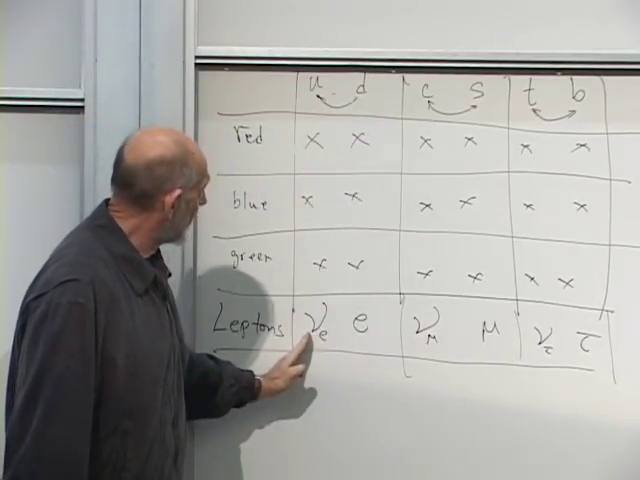
\includegraphics[width=0.82\textwidth]{lecture_05_figure_05.png}
\caption{黒板の表：カラーは赤、青、緑の行の間で作用するのに対し、弱い\(SU(2)\)は対になったフレーバー列とレプトンの行を結びつける。}
\lectureframe{01:03:35}
\end{figure}

レプトンを第4のカラーと呼ぶのは、この段階では単なる類推にすぎない。それらは弱二重項の表の第4行を埋めるが、通常のQCD\(SU(3)\)はクォークをレプトンに回転させない。

\section{荷電弱ゲージボソンの構成}

\subsection{荷電ボソンの量子数}

ゲージボソンは、二重項のある構成要素から別の構成要素へ移るために必要な変換性を担う。レプトン対\(e^-\bar\nu_e\)から始めよう。それは電気電荷\(-1\)を持つので、対応する荷電ゲージボソンは\(W^-\)と呼ばれる。
\begin{equation}
W^-\sim e^-\bar\nu_e.
\end{equation}
同じ量子数はダウンクォークと反アップクォークからも生じる。
\begin{equation}
W^-\sim d\bar u.
\end{equation}
記号\(\sim\)は、同じ関連するゲージ量子数を持つことを意味する。\(W\)が文字通りこれらの粒子の束縛状態であることを意味するのではない。反粒子は共役な組み合わせを持つ。
\begin{equation}
W^+\sim e^+\nu_e\sim\bar d u.
\end{equation}

荷電弱頂点には次が含まれる。
\begin{align}
e^-&\longrightarrow\nu_e+W^-,
&
\mu^-&\longrightarrow\nu_\mu+W^-,
\label{eq:l5-lepton-w}\\
d&\longrightarrow u+W^-,
&
s&\longrightarrow c+W^-,
\label{eq:l5-quark-w}
\end{align}
運動学的に許される場合には第3世代についても同様の遷移がある。ゲージボソンは、対称性が二重項に対して行うのと同じ水平方向の混合を動的に行う。

\begin{classroomqa}
\audiencequestion{電荷保存により、放出されるボソンは電荷\(-1\)を持つように定まるが、なぜ電子、ダウンクォーク、ストレンジクォークの遷移がすべて同じ粒子を関与させなければならないのか。
\lecturetimestamp{01:12:56}}
\lecturerresponse{それは共通の弱い対称性によって記述される経験的事実である。自然は、各世代に、あるいはクォークとレプトンに別々に、異なる\(W\)型ボソンを割り当てても一貫していたであろう。そうではなく、一つの\(SU(2)\)がすべての二重項に同時に作用し、同じ荷電ゲージボソンがこれらすべての遷移を媒介する。}
\end{classroomqa}

\subsection{頂点の読み方と反転}

一つの頂点は過程の族を表す。入射線を出射線に反転させると粒子は反粒子に変わり、\(W^-\)線を反転させると\(W^+\)が得られる。したがって、電荷、運動量、および関連するすべての量子数を一貫して追跡する限り、一つの頂点を放出、吸収、崩壊、対消滅、または逆反応として読むことができる。

\begin{classroomqa}
\audiencequestion{これらの弱い頂点における矢印と線は反転できるのか。
\lecturetimestamp{01:14:51}}
\lecturerresponse{できる。線は終状態から始状態へ、またはその逆に交差させることができるが、その場合粒子は反粒子になる。したがって同じ局所頂点が、多くの異なる向きの反応を記述する。}
\end{classroomqa}

\begin{classroomqa}
\audiencequestion{ストレンジ線とチャーム線を伴う\(W^-\)を書くことは、そのボソンが文字通りストレンジクォークと反チャームクォークの束縛状態であることを意味するのか。
\lecturetimestamp{01:15:43}}
\lecturerresponse{いいえ。線の帳簿付けは、その\(W^-\)がそれらの列の間の量子数の変化を運ぶということだけを述べている。図を崩壊として読むなら、十分に高いエネルギーの\(W^-\)がストレンジクォークと反チャームクォークを生成しうるが、それはそれらから構成されているのではない。}
\end{classroomqa}

\begin{classroomqa}
\audiencequestion{電子と反ニュートリノが\(W\)を作り、それが次にクォーク対を生成できるのか。
\lecturetimestamp{01:17:22}}
\lecturerresponse{そのとおり。十分な重心系エネルギーがあれば、初期のレプトンは荷電カレント中間状態を形成でき、その状態は許されたクォークチャネルを通じて現れうる。二つの頂点は崩壊で用いられたものと同じであり、別の向きに読んだものである。}
\end{classroomqa}

\subsection{欠けている第三のボソン}

\(SU(2)\)群は三つの生成子を持ち、したがって三つのゲージ場を持つ。これまでに示したのは\(W^+\)と\(W^-\)だけである。第三の電気的に中性な場は、電子--陽電子やニュートリノ--反ニュートリノといった量子数のような対角結合に関連付けられなければならない。それは意図的に背景に潜ませてある。物理的な\(Z\)ボソンと光子との関係には電弱混合が必要であり、それは後で扱う。

\begin{classroomqa}
\audiencequestion{弱い力と強い力は異なる歴史的時期に疑われていたのか。
\lecturetimestamp{01:24:11}}
\lecturerresponse{それらの実験的根源は初期の放射能においてともに現れた。アルファ崩壊は核および強い相互作用の物理を明らかにし、ベータ崩壊は弱い相互作用を明らかにし、ガンマ崩壊は電磁光子を放出した。ベクレルの時代には、それらの現代的な場の理論が存在するずっと前に、すでに三つの手がかりすべてが含まれていた。}
\end{classroomqa}

\section{荷電カレント崩壊の演習}

\subsection{パイオン崩壊}

負に帯電したパイオンは価クォーク内容
\begin{equation}
\pi^-=d\bar u.
\end{equation}
を持つ。それらの量子数は\(W^-\)に消滅し、それが次に荷電レプトンと対応する反ニュートリノを生成しうる：
\begin{align}
\pi^-&\longrightarrow W^{-*}
\longrightarrow e^-+\bar\nu_e,
\label{eq:l5-pion-electron}\\
\pi^-&\longrightarrow W^{-*}
\longrightarrow \mu^-+\bar\nu_\mu.
\label{eq:l5-pion-muon}
\end{align}
星印は中間\(W\)が仮想であることを思い出させる。第二のチャネルが主要なものである。

\begin{figure}[htbp]
\centering
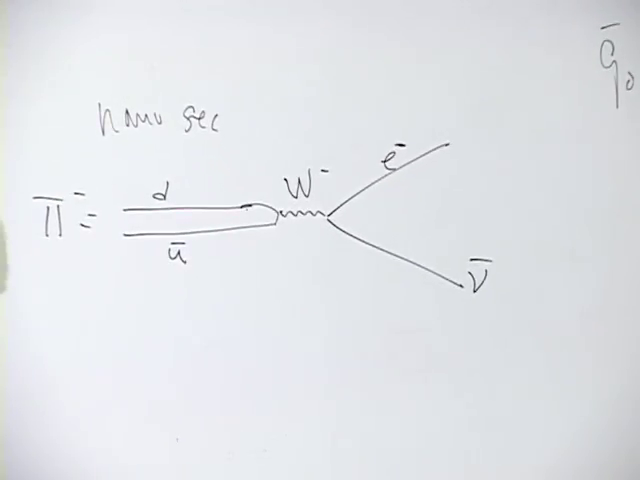
\includegraphics[width=0.72\textwidth]{lecture_05_figure_04.png}
\caption{\(d\bar u\)パイオンが仮想\(W^-\)に消滅し、続いて荷電レプトンとそれに対応する反ニュートリノが生じる。}
\lectureframe{01:19:38}
\end{figure}

\begin{classroomqa}
\audiencequestion{時間の向きが垂直ではなく水平に描かれていても、これは本当にファインマン図なのか。
\lecturetimestamp{01:20:21}}
\lecturerresponse{はい。ページ上での時間の向きは約束事である。一つの向きを時間と宣言し、すべての矢印を一貫して解釈すれば、その図は同じ相互作用の情報を運ぶ。}
\end{classroomqa}

\begin{classroomqa}
\audiencequestion{この図は、不可逆な一方向の崩壊としてよりも、可逆な化学反応のように読めるのではないか。
\lecturetimestamp{01:21:35}}
\lecturerresponse{逆過程は許されている。真空中で生成されたパイオンが崩壊するのは、出射粒子が離れていき、通常は再結合しないからである。しかし、ミューオンと反ニュートリノが適切なエネルギーと運動量で一緒に打ち込まれれば、逆の相互作用を通じてパイオンを形成する非零の振幅が存在する。}
\end{classroomqa}

\subsection{エネルギーと仮想中間状態}

静止しているパイオンについては、
\begin{equation}
m_\pi\simeq140\ {\rm MeV},
\qquad
m_\mu\simeq106\ {\rm MeV},
\qquad
m_\nu\approx0
\end{equation}
ここで問題となる精度では成り立つ。残りのエネルギーは出ていく粒子の運動エネルギーになる。運動量保存則により
\begin{equation}
\boldsymbol p_\mu+\boldsymbol p_{\bar\nu}=0,
\end{equation}
が要求されるので、2つの粒子はパイオン静止系で背中合わせに飛び去る。

\begin{classroomqa}
\audiencequestion{中間状態の\(W\)がパイオンよりはるかに重いのに、どうしてエネルギーは保存されるのですか。
\lecturetimestamp{01:25:08}}
\lecturerresponse{初期状態と終状態の粒子だけが質量殻上になければならない。四元運動量は各頂点で保存されるが、内部の仮想線は\(E^2=\boldsymbol p^2+m_W^2\)に従う必要はない。そのオフシェルからのずれが大きいほど、その伝播関数は過程をより強く抑制する。\editorialnote{講義では伝統的なエネルギー--時間の不確定性の言葉遣いを用い、中間状態は短時間エネルギーを破ってよいと述べている。現代的な正確な言明は回答にあるとおりである。すなわち、エネルギー・運動量は保存され、仮想の内部線は実粒子の質量殻条件を満たす必要はない。}}
\end{classroomqa}

\subsection{ミューオン崩壊}

ミューオンはまず仮想\(W^-\)を放出して自身のニュートリノに変わりうる：
\begin{equation}
\mu^-\longrightarrow\nu_\mu+W^{-*}.
\end{equation}
次にその仮想ボソンが電子と電子反ニュートリノを生成する：
\begin{equation}
\mu^-\longrightarrow
\nu_\mu+e^-+\bar\nu_e.
\label{eq:l5-muon-decay}
\end{equation}
これは純粋にレプトン的な過程である。ミューオンは電子より約200倍重いので、終状態の静止質量を差し引いても十分な運動エネルギーが残る。

\begin{figure}[htbp]
\centering
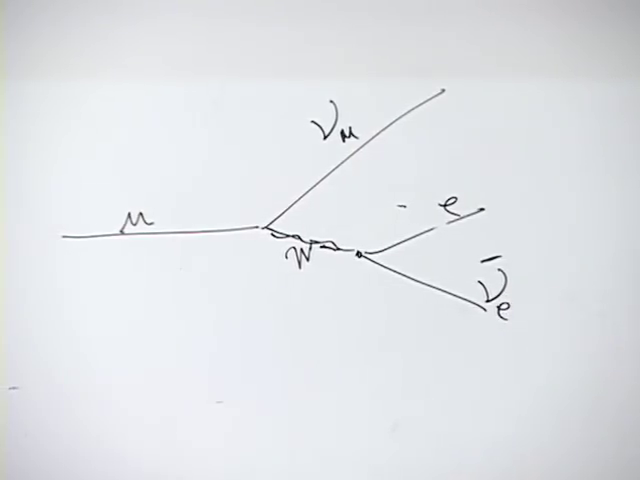
\includegraphics[width=0.72\textwidth]{lecture_05_figure_06.png}
\caption{仮想荷電弱ゲージボソンを介したミューオン崩壊。}
\lectureframe{01:29:24}
\end{figure}

\begin{classroomqa}
\audiencequestion{電子とともに放出される中性粒子は反ニュートリノですか。
\lecturetimestamp{01:29:06}}
\lecturerresponse{はい。完全な終状態には1個のミューニュートリノ、1個の電子反ニュートリノ、そして電子が含まれる。フレーバーのラベルを保つことで、2つの中性粒子を混同せずに済む。}
\end{classroomqa}

電子はミューオンより軽いので、真空中でこの崩壊を逆向きに進めることはできない。タウはより重く、同様の弱いチャネルを通じて崩壊できる。ここでの安定性は部分的には質量順序の偶然であり、基礎となる頂点の違いではない。

\begin{classroomqa}
\audiencequestion{線形加速器は事実上電子の質量を増やし、それによって本来禁止されている反応を逆方向に進行させることができるのですか。
\lecturetimestamp{01:30:23}}
\lecturerresponse{電子の不変な静止質量は変わらないが、運動エネルギーを与える。十分な重心系エネルギーがあればより重い終状態粒子を生成できるので、質量を利用可能な衝突エネルギーに置き換えれば、提案された物理的考えは正しい。}
\end{classroomqa}

\subsection{クォークレベルでの中性子ベータ崩壊}

中性子と陽子の価クォーク組成は
\begin{equation}
n=udd,
\qquad
p=uud.
\end{equation}
中性子中の1個のダウンクォークが荷電カレント遷移
\begin{equation}
d\longrightarrow u+W^{-*},
\end{equation}
を起こし、\(udd\)を\(uud\)に変える。次に仮想ボソンが崩壊する：
\begin{equation}
W^{-*}\longrightarrow e^-+\bar\nu_e.
\end{equation}
2つの頂点を組み合わせると
\begin{equation}
n\longrightarrow p+e^-+\bar\nu_e.
\end{equation}
が再現される。

逆のクォーク遷移\(u\to d+W^+\)は3個のダウンクォークからなるバリオンを残すが、その利用可能な状態は自由中性子が生成するには重すぎる。実際のダウンからアップへの経路がエネルギー的に許される経路である。

\begin{classroomqa}
\audiencequestion{中性子は代わりに陽子、ミューオン、および対応する反ニュートリノに崩壊できますか。
\lecturetimestamp{01:32:38}}
\lecturerresponse{静止した自由中性子では不可能である。中性子--陽子の質量差はミューオンの質量よりはるかに小さい。十分な追加の衝突エネルギーまたは励起エネルギーがあれば、同じ弱い頂点がミューオンを生成するチャネルに関与しうる。この禁止は運動学的なものであり、相互作用の欠如ではない。}
\end{classroomqa}

\section{未解決の抑制}

荷電弱頂点はどの過程が起こりうるかを説明するが、なぜそれらがそれほど遅いかはまだ説明しない。魅力的な答えの一つは、異常に小さな弱結合である。その答えは誤りである。無次元の弱ゲージ結合はほぼ電磁気的な大きさである。抑制は別の何かから来なければならない。

欠けている要素はすでに仮想伝播関数に見えている。すなわち\(W\)が非常に重いのである。\(m_W\)よりはるかに低いエネルギーでは、荷電カレント振幅はほぼ\(1/m_W^2\)の冪で抑制される。この関連は、ヒッグス機構と電弱対称性の破れがゲージボソンがいかに質量を獲得するかを説明した後に展開される。
\editorialnote{講義ではこれを次回の謎として残している。重い\(W\)による説明は前方へのつながりとしてここに含めたものであり、その導出がこの講義で行われたという主張ではない。}

\begin{classroomqa}
\audiencequestion{この理論がこの対称性をもつと言うとき、対応する操作の下でそのラグランジアンが不変であるという意味だろうか。
\lecturetimestamp{01:34:14}}
\lecturerresponse{そのとおりである。理論がこの対称性をもつという主張は、それらの変換の下でのラグランジアン、あるいは同等に作用の不変性を略して述べたものである。完全なラグランジアンを書くことは後回しにされているのであって、別の定義に置き換えられているのではない。}
\end{classroomqa}

これで道筋は完成した。マクスウェル理論が原型を与え、QCDは非可換ゲージボソンが電荷を運び交換する仕組みを示し、結合定数は原子とハドロンの時間スケールの対比を説明し、そして弱い\(SU(2)\)はクォークとレプトンを\(W^\pm\)で結ばれた二重項へと組織する。残された課題は、これらのゲージ媒介過程が、その根底にある結合が格別小さいわけではないにもかかわらず、実際にはなぜ弱いのかを理解することである。